\usetikzlibrary{arrows}
\usetikzlibrary{decorations.pathreplacing}

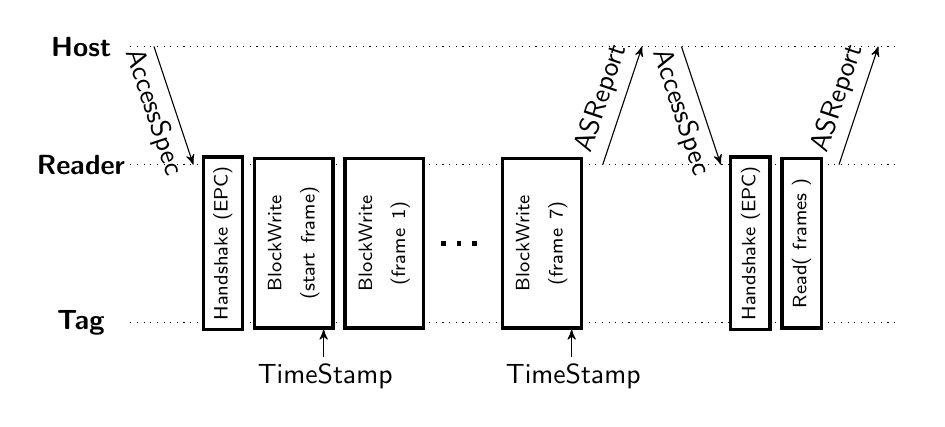
\begin{tikzpicture}[font=\sffamily,
>=stealth',
commentl/.style={text width=3cm},
scale=1.0, 
every node/.style={scale=1.0}]
\tikzstyle{bl} = [draw,rotate=90,minimum height=5mm,minimum width=21.5mm, very thick, draw=black, top color=white]
\tikzstyle{BL} = [draw,rotate=90,minimum height=10mm,minimum width=21.5mm, very thick, draw=black, top color=white,text width=1.8cm,align=center]

\node(host) at (0.5,3.5cm){\textbf{Host}};
\node(reader) at (0.5,2cm){\textbf{Reader}};
\node(tag) at (0.5,0cm){\textbf{Tag}};
\node(h) at (0,3.5cm){};
\node(r) at (0,2cm){};
\node(t) at (0,0cm){};

\foreach \x in {0,2cm,3.5cm}{
	\node (v1) at (10mm,\x) {};	
	\node (v2) at (110mm,\x) {};
	\draw [dotted] (v1) edge (v2);
}

\draw[->] ([xshift=13mm]h.east)  --
([xshift=18mm]r.east)node[midway, below, sloped]     { AccessSpec};

\node[bl](x) at (2.3cm,1cm){\scriptsize{Handshake (EPC)}};
\node[BL](b0) at ([xshift=9mm]x){\scriptsize{BlockWrite (start frame)}};
\node[BL](x) at ([xshift=11.5mm]b0){\scriptsize{BlockWrite (frame 1)}};

\node[BL](b7) at ([xshift=20mm]x){\scriptsize{BlockWrite (frame 7)}};
\draw[loosely dotted,ultra thick] ([xshift=2mm]x.south) --([xshift=-2mm]b7.north);

\draw[->] ([xshift=70mm]r.east)--
([xshift=75mm,yshift=1.5cm]r.east) node[midway, above, sloped] { ASReport};

\draw[->] ([xshift=80mm]h.east)  --
([xshift=85mm]r.east) coordinate(as2) node[midway, below, sloped]     { AccessSpec};
\node[bl](x) at (90mm,1cm){\scriptsize{Handshake (EPC)}};
\node[bl](x) at ([xshift=6.5mm]x){\scriptsize{Read( frames )}};
\draw[->] ([xshift=15mm]as2.east)--
([xshift=20mm,yshift=1.5cm]as2.east) node[midway, above, sloped] { ASReport};

%\tikzstyle{br} = [decorate, decoration={brace, amplitude=4pt}]
%\draw[br] ([xshift=19mm]t.east) -- ([xshift=13mm]t.east) node[midway, , sloped,yshift=-6mm] {Other slots};
%\draw[br] ([xshift=49mm]t.east) -- ([xshift=43mm]t.east) node[midway, , sloped,yshift=-6mm] {Other slots};
% Timestamp stuff:
\node(tTag) at ([yshift=-6mm,xshift=4mm]b0.west){TimeStamp};
\draw[->] ([yshift=2.5mm,xshift=-10mm]tTag.east)--([yshift=6mm,xshift=-10mm]tTag.east) node[near start]     {};

\node(tTag) at ([yshift=-6mm,xshift=4mm]b7.west){TimeStamp};
\draw[->] ([yshift=2.5mm,xshift=-10mm]tTag.east)--([yshift=6mm,xshift=-10mm]tTag.east) node[near start]     {};

\end{tikzpicture}